\documentclass[12pt]{article}
	
\usepackage[a4paper, margin=1cm]{geometry}
\usepackage[table]{xcolor}
\usepackage{graphicx}
\usepackage{tabularx}
\usepackage{array}
\newcommand\topspace{0.2cm}
\newcommand\bottomspace{0.3cm}
\newcommand\ttpadt{0.1cm}
\newcommand\ttpadb{0.1cm}
\newcommand\sep{\vspace{\bottomspace}\noindent\hrulefill\vspace{\topspace}}


\pagenumbering{gobble}

\title{CHEATSHEET}
\author{Simon Pauw}

\begin{document}

\noindent\hrulefill\vspace{0.6cm}


\centering\textbf{\large PIDAC Cheatsheet - Week 1} 


\sep


\renewcommand{\arraystretch}{1.4}
\noindent
\begin{tabularx}{\textwidth}{l>{\centering\arraybackslash}m{4cm}>{\centering\arraybackslash}m{4cm}>{\centering\arraybackslash}m{4cm}c}

\textbf{Poort} & \textbf{Rechthoekige notatie} & \textbf{Alternatieve notatie} & \textbf{Waarheidstabel} & \textbf{Boole algebra} \\
\hline
AND & 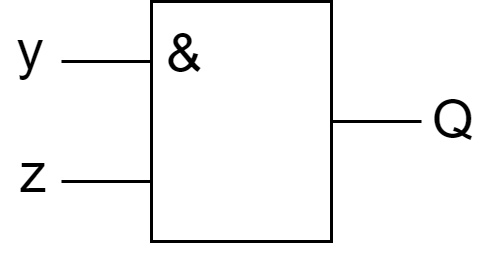
\includegraphics[width=3cm]{images/AND.png} & 
\includegraphics[width=3cm]{images/dist_AND.png} & \vspace{\ttpadt} \raisebox{0.8\height}{$
\begin{array}{cc|c}
y & z & Q \\
\hline
0 & 0 & 0 \\
0 & 1 & 0 \\
1 & 0 & 0 \\
1 & 1 & 1 \\
\end{array}$} \vspace{\ttpadb}
 & \( Q = y \cdot z \) \\

OR & 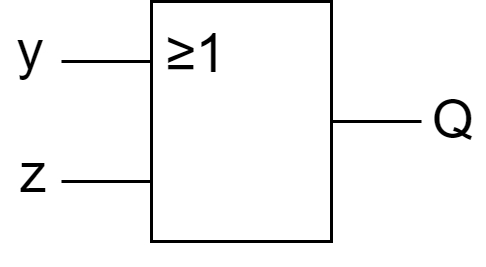
\includegraphics[width=3cm]{images/OR.png} & 
\includegraphics[width=3cm]{images/dist_OR.png} & \vspace{\ttpadt} \raisebox{0.8\height}{$
\begin{array}{cc|c}
y & z & Q \\
\hline
0 & 0 & 0 \\
0 & 1 & 1 \\
1 & 0 & 1 \\
1 & 1 & 1 \\
\end{array}$} \vspace{\ttpadb} & \( Q = y + z \) \\

XOR & 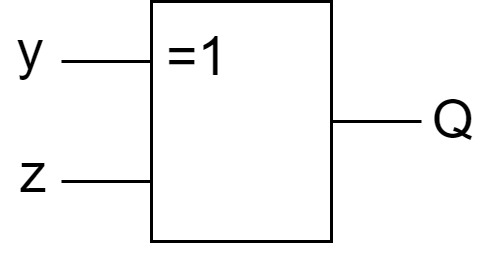
\includegraphics[width=3cm]{images/XOR.png} & 
\includegraphics[width=3cm]{images/dist_XOR.png} & \vspace{\ttpadt} \raisebox{0.8\height}{$
\begin{array}{cc|c}
y & z & Q \\
\hline
0 & 0 & 0 \\
0 & 1 & 1 \\
1 & 0 & 1 \\
1 & 1 & 0 \\
\end{array}$} \vspace{\ttpadb} & \( Q = y \oplus z \) \\

Inverter & \includegraphics[width=3cm]{images/Inverter.png} & 
\includegraphics[width=3cm]{images/dist_inverter.png} &  \vspace{\ttpadt} \raisebox{0.8\height}{$
\begin{array}{c|c}
y & Q \\
\hline
0 & 1 \\
1 & 0 \\
\end{array}$} \vspace{\ttpadb}& \( Q = \overline{y} \) \\

NAND & 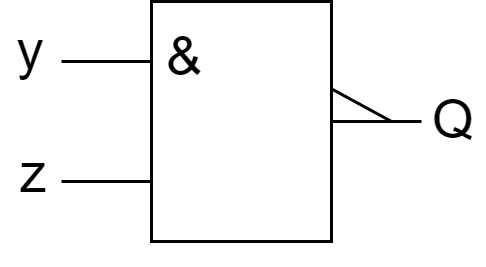
\includegraphics[width=3cm]{images/NAND.png} & 
\includegraphics[width=3cm]{images/dist_NAND.png} & \vspace{\ttpadt} \raisebox{0.8\height}{$
\begin{array}{cc|c}
y & z & Q \\
\hline
0 & 0 & 1 \\
0 & 1 & 1 \\
1 & 0 & 1 \\
1 & 1 & 0 \\
\end{array}$} \vspace{\ttpadb} & \( Q = \overline{y \cdot z} \) \\

NOR & 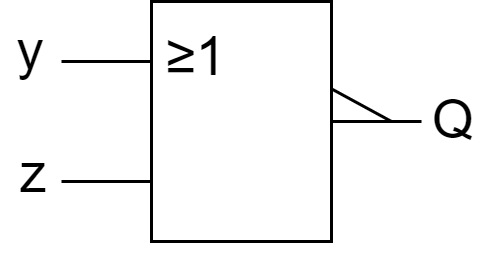
\includegraphics[width=3cm]{images/NOR.png} & 
\includegraphics[width=3cm]{images/dist_NOR.png} & \vspace{\ttpadt} \raisebox{0.8\height}{$
\begin{array}{cc|c}
y & z & Q \\
\hline
0 & 0 & 1 \\
0 & 1 & 0 \\
1 & 0 & 0 \\
1 & 1 & 0 \\
\end{array}$} \vspace{\ttpadb} & \( Q = \overline{y + z} \) \\
\hline
\end{tabularx}

\pagebreak

\noindent\hrulefill\vspace{0.6cm}


\centering\textbf{\large PIDAC Cheatsheet - Week 2} 


\sep


\textbf{Rekenregels}\\

\[
\begin{array}{rccc}
1. & z + z &=& z        \\                  
2. & z \cdot z &=& z    \\              
3. & \overline{\overline{z}} &=& z \\
4. & z + \overline{z} &=& 1           \\
5. & z \cdot \overline{z} &=& 0    \\
6. &\overline{0} &=& 1 \\
7. & \overline{1} &=& 0 \\
8. & z + 0 &=& z     \\
9. & z + 1 &=& 1    \\
10. & z \cdot 0 &=& 0 \\
11. & z \cdot 1 &=& z
\end{array}
\]

\sep

\textbf{Associativiteit}\\

\[
\begin{array}{lccc}
12. & (x + y) + z &=& x + (y + z) \\
13. & (x \cdot y) \cdot z &=& x \cdot (y \cdot z)
\end{array}
\]

\sep 

\textbf{Commutativiteit}\\

\[
\begin{array}{lccc}
14. & y + z &=& z + y \\
15. & y \cdot z &=& z \cdot y
\end{array}
\]

\sep

\textbf{Distributieve wetten}\\

\[
\begin{array}{lccc}
16. & x \cdot y + x \cdot z &=& x \cdot (y + z) \\
17. & (x + y) \cdot (x + z) &=& x + y \cdot z 
\end{array}
\]

\sep

\textbf{Absorptie, De Morgan en XOR}\\

\[
\begin{array}{lccc}
18. & y + \overline{y} \cdot z &=& y + z\\
19. & \overline{y \cdot z} &=& \overline{y} + \overline{z} \\
20. & y \cdot \overline{z} + \overline{y} \cdot{z} & = & y \oplus z
\end{array}
\]

\vspace{\bottomspace}\noindent\hrulefill


\end{document}